\section{Beispiele}

% Erwachsener/Kind
\begin{frame}
    \frametitle{Relationaler Datensatz mit Arrays?}

    \begin{columns}[T,onlytextwidth]
        \column{0.475\textwidth}
            \begin{table}
                \centering
                \begin{adjustbox}{width=\textwidth}
                    \small
                    \begin{tabular}[c]{|c|c|c|c|c}

                        \hline

                        \multicolumn{1}{|c|}{\textbf{id}} &
                        \multicolumn{1}{c|}{\textbf{name}} &
                        \multicolumn{1}{c|}{\textbf{vorname}} &
                        \multicolumn{1}{c|}{\textbf{alter}} &
                        \multicolumn{1}{c}{\dots} \\

                        \multicolumn{1}{|c|}{\textit{int}} &
                        \multicolumn{1}{c|}{\textit{String}} &
                        \multicolumn{1}{c|}{\textit{String}} &
                        \multicolumn{1}{c|}{\textit{int}} &
                        \multicolumn{1}{c}{\dots} \\

                        \hline

                        0  & Mustermann  & Max    & 27             & \dots \\
                        1  & Mustermann  & Marie  & 26             & \dots \\
                        2  & Fröhlich    & Nico   & 18             & \dots \\
                        3  & Hammer      & Niko   & \textit{null}  & \dots \\
                        $\vdots$ & $\vdots$ & $\vdots$ & $\vdots$ &

                    \end{tabular}
                \end{adjustbox}
                \caption{Datensatz \say{Erwachsene} als relationale Datenbank}
                \label{tab:erwachsene1}
            \end{table}

        \pause

        \column{0.475\textwidth}
        \begin{table}
            \centering
            \begin{adjustbox}{width=\textwidth}
                \small
                \begin{tabular}[c]{|c|c|c|c|c}

                    \hline

                    \multicolumn{1}{|c|}{\textbf{id}} &
                    \multicolumn{1}{c|}{\textbf{name}} &
                    \multicolumn{1}{c|}{\textbf{vorname}} &
                    \multicolumn{1}{c|}{\textbf{alter}} &
                    \multicolumn{1}{c}{\dots} \\

                    \multicolumn{1}{|c|}{\textit{int}} &
                    \multicolumn{1}{c|}{\textit{String}} &
                    \multicolumn{1}{c|}{\textit{String}} &
                    \multicolumn{1}{c|}{\textit{int}} &
                    \multicolumn{1}{c}{\dots} \\

                    \hline

                    0  & Mustermann  & John   & 8   & \dots \\
                    1  & Mustermann  & Jan    & 3   & \dots \\
                    2  & Mustermann  & Phil   & 5   & \dots \\
                    3  & Hammer      & Paul   & 1   & \dots \\
                    $\vdots$ & $\vdots$ & $\vdots$ & $\vdots$ &

                \end{tabular}
            \end{adjustbox}
            \caption{Datensatz \say{Kinder} als relationale Datenbank}
            \label{tab:kinder1}
        \end{table}

    \end{columns}
\end{frame}

% Arrays
\begin{frame}
    \frametitle{Relationaler Datensatz mit Arrays?}

    \begin{table}
        \centering
        \begin{adjustbox}{width=\textwidth}
            \small
            \begin{tabular}[c]{|c|c|c|c|c|c}

                \hline

                \multicolumn{1}{|c|}{\textbf{id}} &
                \multicolumn{1}{c|}{\textbf{name}} &
                \multicolumn{1}{c|}{\textbf{vorname}} &
                \multicolumn{1}{c|}{\textbf{alter}} &
                \multicolumn{1}{c|}{\textbf{kinder}} &
                \multicolumn{1}{c}{\dots} \\

                \multicolumn{1}{|c|}{\textit{int}} &
                \multicolumn{1}{c|}{\textit{String}} &
                \multicolumn{1}{c|}{\textit{String}} &
                \multicolumn{1}{c|}{\textit{int}} &
                \multicolumn{1}{c|}{\textbf{int[]?}} &
                \multicolumn{1}{c}{\dots} \\

                \hline

                0  & Mustermann  & Max    & 27            & [0,1,2]?       & \dots \\
                1  & Mustermann  & Marie  & 26            & [0]?           & \dots \\
                2  & Fröhlich    & Nico   & 18            & \textit{null}  & \dots \\
                3  & Hammer      & Niko   & \textit{null} & [3]            & \dots \\
                $\vdots$ & $\vdots$ & $\vdots$ & $\vdots$ & $\vdots$ &

            \end{tabular}
        \end{adjustbox}
        \caption{Theoretischer Datensatz \say{Erwachsene} als relationale Datenbank}
        \label{tab:erwachsene2}
    \end{table}

\end{frame}

\begin{frame}
    \frametitle{Relationaler Datensatz mit Objekten?}
    % minted kinda doesnt want to compile in the beamer environment so i have to use this bad alternative which makes me sad. verbatim doesnt work either for some stupid reason.
    \begin{figure}
        \begin{small}
            \begin{center}
                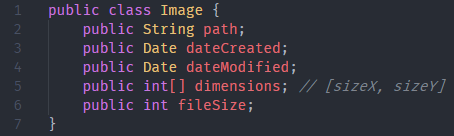
\includegraphics[width=0.95\textwidth]{img/ClassExample.png}
            \end{center}
            \caption{Beispiel einer \say{Image} Klasse}
            \label{fig:image}
        \end{small}
    \end{figure}
\end{frame}

\begin{frame}
    \frametitle{Relationaler Datensatz mit Objekten?}

    \begin{table}
        \centering
        \begin{adjustbox}{width=\textwidth}
            \small
            \begin{tabular}[c]{|c|c|c|c|c|c}

                \hline

                \multicolumn{1}{|c|}{\textbf{id}} &
                \multicolumn{1}{c|}{\textbf{name}} &
                \multicolumn{1}{c|}{\textbf{vorname}} &
                \multicolumn{1}{c|}{\textbf{alter}} &
                \multicolumn{1}{c|}{\textbf{portrait}} &
                \multicolumn{1}{c}{\dots} \\

                \multicolumn{1}{|c|}{\textit{int}} &
                \multicolumn{1}{c|}{\textit{String}} &
                \multicolumn{1}{c|}{\textit{String}} &
                \multicolumn{1}{c|}{\textit{int}} &
                \multicolumn{1}{c|}{\textbf{Image}} &
                \multicolumn{1}{c}{\dots} \\

                \hline

                0  & Mustermann  & Max    & 27             & <Instanz>      & \dots \\
                1  & Mustermann  & Marie  & 26             & <Instanz>      & \dots \\
                2  & Fröhlich    & Nico   & 18             & \textit{null}  & \dots \\
                3  & Hammer      & Niko   & \textit{null}  & <Instanz>     & \dots \\
                $\vdots$ & $\vdots$ & $\vdots$ & $\vdots$ & $\vdots$ &

            \end{tabular}
        \end{adjustbox}
        \caption{\say{Erwachsene}\dots mit Bildern?}
        \label{tab:erwachsene3}
    \end{table}

\end{frame}
